%%%%%%%%%%%%%%%%%%%%%%%%%%%%%%%%%%%%%%%%%%%%%%%%%%%%%%%%%%%%%%%%%%%%%%%%%%%%%%
%
% タイトル TeX用テンプレート 
% バージョン 2014-11-8 (Sat) 初版
% 作成者 Kouhei Ito
% 作成場所 野々市市中林 DeuxMKK
% 用途 2段組レポートの作成等
%
%%%%%%%%%%%%%%%%%%%%%%%%%%%%%%%%%%%%%%%%%%%%%%%%%%%%%%%%%%%%%%%%%%%%%%%%%%%%%%%%
%\documentclass[11pt,twocolumn]{jsarticle}
\documentclass[11pt]{jsarticle}
\usepackage[dvipdfmx]{graphicx}
\usepackage{amsmath,amssymb}
\usepackage{url}
\usepackage{nidanfloat}

%% 体裁

% ページレイアウト(A4:297 mm × 210 mm,1 インチ = 25.4 mm)
% http://www.biwako.shiga-u.ac.jp/sensei/kumazawa/tex/layout.html
% http://www.slis.tsukuba.ac.jp/~fujisawa.makoto.fu/cgi-bin/wiki/index.php?TeX%A5%E1%A5%E2#p61e1b46
% 上 20 mm,下 22 mm,左右 20 mm の余白設定
\setlength{\topmargin}{-20truemm}
\setlength{\headheight}{10truemm}
\setlength{\headsep}{4.6truemm}
\setlength{\textheight}{255truemm}
\setlength{\oddsidemargin}{-5.4truemm}
\setlength{\evensidemargin}{-5.4truemm}  % twoside オプション指定時のみ有効
\setlength{\textwidth}{170truemm}
% \setlength{\columnsep}{8truemm}
\setlength{\columnsep}{6truemm}


%%%%%%%%%%%%%%%%%%%%%%%%%%%%%%%%%%%%%%%%%%%%%%%%%%%%%%%%%%%%%%%%%%%%%%%%%%%%%%%%
\title{モーター特性の実験}
\author{金沢工業高等専門学校 北山,剱崎}
\date{2016-9-1}
%%%%%%%%%%%%%%%%%%%%%%%%%%%%%%%%%%%%%%%%%%%%%%%%%%%%%%%%%%%%%%%%%%%%%%%%%%%%%%%%
\begin{document}
\maketitle
%\begin{abstract}
%ボルダの振り子を用いて重力加速度を測定した.
%得られた値は,$g=9.80 \pm 0.02 [\textrm{m}/\textrm{sec}^2]$であった.
%\end{abstract}

%\tableofcontents
%%%%%%%%%%%%%%%%%%%%%%%%%%%%%%%%%%%%%%%%%%%%%%%%%%%%%%%%%%%%%%%%%%%%%%%%%%%%%%%%

要項

制御実験機のモーターの挙動が均一でないため,それぞれのモーターの特性を確認する実験を行った.
実験の手順を以下に示す.

(1)モーター1(R)から4(F)の順に10秒間かけて指令値を1.0msから2.0msまで徐々に上げていく.

(2)同時にジャイロセンサを振動センサ代わりにし,指令値とモーターの回り始めを検出する.

(3)gnuplotを用いてグラフ化する.


結果

上記の実験を行った結果得られたグラフを図\ref{fig:chara}に示す.
振動gzが小さい時,回転は弱い.モーターR,Fが振動が大きく,L,Fがモーターの回り始めが遅いことがわかる.


考察

実際のプログラムでドローンを飛ばす際始動が遅れている分予め指令値の値を引き上げておくことで,垂直に離陸できない問題が改善されるのではないかと考えられる.


\begin{figure*}[b]
 \begin{center}
  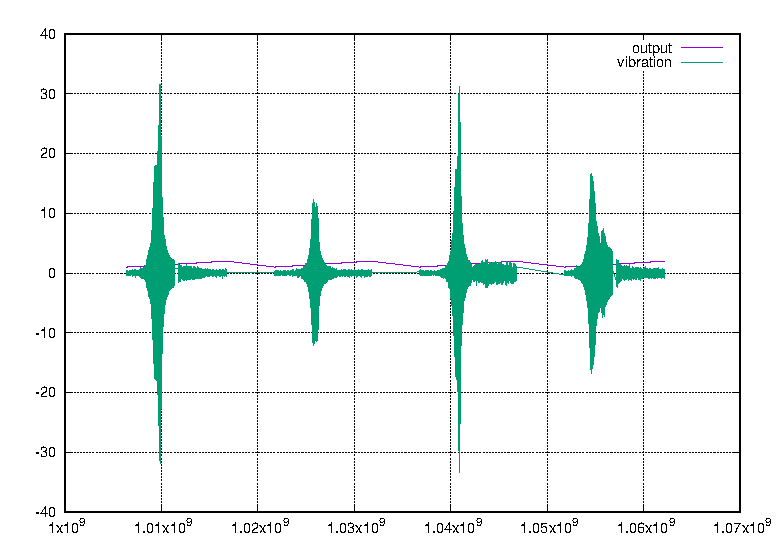
\includegraphics[width=130mm]{motor_chara.eps}
  \caption{モーターの特性}
  \label{fig:chara}
 \end{center}
\end{figure*}

%%%%%%%%%%%%%%%%%%%%%%%%%%%%%%%%%%%%%%%%%%%%%%%%%%%%%%%%%%%%%%%%%%%%%%%%%%%%%%%%


\end{document}
